
\documentclass[xcolor={usenames,dvipsnames},12pt,presentation,aspectratio=169]{beamer}

\usepackage[utf8]{inputenc}
\usepackage{fontawesome}
\usepackage[brazilian]{babel}
\usepackage{verbatim}
\usepackage{graphicx}
\usepackage{xspace}
\usepackage{amsthm}
\usepackage{url}
\usepackage{array}
\usepackage{hyperref}
\usepackage{times,mathptmx}
\usepackage{pdfpages}
\usepackage{mdframed}
\usepackage{tikz}
\usepackage{alltt}
\usepackage{minted}
%\usepackage{times}
%\usepackage[usenames,dvipsnames]{xcolor}
%\usepackage[usenames,dvipsnames]{color}
%\usepackage{color}

\usetikzlibrary{arrows,shapes}

\usetheme{Madrid}
%\usetheme{Boadilla}
%\usetheme{Darmstadt}
%\usetheme{Frankfurt}
%\usetheme{CambridgeUS}
%\usetheme{AnnArbor}
%\usecolortheme{beaver}
%\usecolortheme{seahorse}
%\usecolortheme{seagull}
\usecolortheme[named=BrickRed]{structure}

\setbeamercovered{transparent}

\setbeamertemplate{footline}[frame number]
%\setbeamertemplate{navigation symbols}{}
%\setbeamersize{text margin left=1em,text margin right=1em}

\newcommand{\titulo}{Programação Paralela com MPI}
\newcommand{\disciplina}{ELC139 - Programação Paralela}
\newcommand{\nome}{João Vicente Ferreira Lima (UFSM)}

\lecture[1]{\aula}{aula01}
\def\lecturename{\aula}

\newcommand{\Red}[1]{{\color{red}#1}}
\newcommand{\red}[1]{{\color{red}#1}}
\newcommand{\Blue}[1]{{\color{blue}#1}}
\newcommand{\blue}[1]{{\color{blue}#1}}

\newcommand{\PBS}[1]{\let\temp=\\#1\let\\=\temp}
\newcommand{\RRCOL}{\PBS\raggedright\hspace{0pt}}

\newcommand{\p}[1]{\texttt{#1}}
\newenvironment{code}{%
  \begin{alltt}%
  }{%
  \end{alltt}%
}

\makeatletter
%\setbeamertemplate{headline}{}
% {%
%   \leavevmode%
%   \@tempdimb=2.4375ex%
%   \ifnum\beamer@subsectionmax<\beamer@sectionmax%
%     \multiply\@tempdimb by 4%
%   \else%
%     \multiply\@tempdimb by\beamer@subsectionmax%
%   \fi%
%   \ifdim\@tempdimb>0pt%
%     \advance\@tempdimb by 1.125ex%
%     \begin{beamercolorbox}[wd=.5\paperwidth,ht=\@tempdimb]{section in head/foot}%
%       \vbox to\@tempdimb{\vfil\insertsectionnavigation{.5\paperwidth}\vfil}%
%     \end{beamercolorbox}%
%     \begin{beamercolorbox}[wd=.45\paperwidth,ht=\@tempdimb]{subsection in head/foot}%
%       \vbox
%       to\@tempdimb{\vfil\insertsubsectionnavigation{.45\paperwidth}\vfil}%
%     \end{beamercolorbox}%
%     \begin{beamercolorbox}[wd=.05\paperwidth,ht=\@tempdimb]{subsection in head/foot}%
%       \vbox
%       to\@tempdimb{\vfil\hfil\insertframenumber\vfil\vfil}%
%     \end{beamercolorbox}%
%   \fi%
% }

\def\dohead{\beamer@headcounter=4\relax\beamer@headcounter=1\loop\ifnum\beamer@headcounter<\beamer@totalheads%
  \advance\beamer@headcounter by1\relax%
  \csname @@head\the\beamer@headcounter\endcsname\repeat}

\makeatother

\title[\titulo]{\titulo}

\subtitle{\disciplina}

\author[João V. F. Lima]{\nome}

%\institute[UFSM]{Departamento de Linguagens e Sistemas de Computação \\ Universidade Federal de Santa Maria \\ \url{jvlima@inf.ufsm.br} \\ \url{http://www.inf.ufsm.br/~jvlima}}
\institute[UFSM]{Universidade Federal de Santa Maria \\ \url{jvlima@inf.ufsm.br} \\ \url{http://www.inf.ufsm.br/~jvlima}}
\date{2023/1}

\graphicspath{{.}{figs/}}

\logo{ 
\includegraphics[height=1.5cm,width=1.5cm,keepaspectratio]{logo_inf}    
        
\includegraphics[height=1.5cm,width=1.5cm,keepaspectratio]{logo_ufsm} }

%\titlegraphic{
%	
\includegraphics[width=2cm]{logo_ufsm}
%  \hspace{1cm}
%	
\includegraphics[width=2cm]{logo_inf}
%}

\newtheorem{mydef}{Definição}[section]
%\newtheorem{myteo}{Teorema}[section]
%------------------------------------------------------------------------------
%\newcommand{\xkaapi}{XKaapi\xspace}
%------------------------------------------------------------------------------
% Typesetting Listings
\usepackage{listings}
\lstset{
  language=C,
  %basicstyle=\scriptsize\ttfamily,
  %basicstyle=\normalsize\ttfamily,
  basicstyle=\small\ttfamily,
  %basicstyle=\footnotesize\ttfamily,
  %aboveskip=0pt,
  %belowskip=0pt,
  %mathescape=false,
  columns=fullflexible,
  %numbers=none,
  numbers=left,
  numbersep=5pt,
%  showtabs=true,
%  showspaces=true,
  frame=tb,
  breaklines=true
}
%------------------------------------------------------------------------------
%\lstset{commentstyle=\color{blue}}
%\lstset{stringstyle=\ttfamily}
%\lstset{ classoffset=1, 
%            morekeywords={kaapi,omp,task,data,alloca, declare, reduction, identity, parallel,sync,taskwait,cilk,spawn,tbb,css,cilk\_spawn,cilk\_sync,cilk\_for,offload},
%            keywordstyle=\color{Red}\bfseries
%           }
%\lstset{ classoffset=2, 
%            morekeywords={value,read,write,readwrite,reduction,untied,firstprivate,TaskBodyCPU,TaskBodyGPU,ka,Signature,RW,CW,range2d\_r,range2d\_rw,range2d,Spawn,Fork,Shared\_w,Shared\_r,Shared,a1,target,device,copyin,copyout,input,implements,copy\_deps,RPWP,range2d\_rpwp,rangeindex,Memory,Register,SetStaticSched,Sync,Unregister,Community,System,join\_community,SpawnMain,leave,initialize,terminate,logfile,array,SetArch,ArchHost,ArchCUDA,W,R,gpuStream,pointer\_w,pointer\_r,pointer\_cw,pointer},
%            keywordstyle=\color{Blue}\bfseries
%           }
%\lstset{ classoffset=3, 
%            morekeywords={storage,ld},
%            keywordstyle=\bfseries
%           }
%\lstset{ classoffset=4, 
%            morekeywords={in,out,inout,cout,concurrent},
%            keywordstyle=\color{Red}\bfseries
%           }
%           
%\lstset{classoffset=0, showstringspaces=false}
%------------------------------------------------------------------------------
\mdfsetup{
  backgroundcolor=gray!10,
%  roundcorner=10pt,
}
%------------------------------------------------------------------------------
\newcommand{\restorefootline}{\setbeamertemplate{navigation symbols}{}}
%\newcommand{\setfootline}[1]{\setbeamertemplate{navigation symbols}{\textcolor{black}{\textbf{#1}}}}
\newcommand{\includeslides}[4]{%
%  \setfootline{#1}%
  {
    \setbeamercolor{background canvas}{bg=}
    \includepdf[pages={#1},%
    pagecommand={},
%    pagecommand={\begin{frame}[default]{}\end{frame}},
%    #4,%
    turn=false,noautoscale=false,column=false,columnstrict=false,openright=false,frame=false]{#2}%
  }
  %\restorefootline%
}
%------------------------------------------------------------------------------
\begin{document}

\begin{frame}
%  \titlepage
  \maketitle
%  \mode<presentation>
%  {
%    \begin{columns}
%      \begin{column}{0.5\textwidth}
%      \raggedleft
%	
\includegraphics[width=2cm]{logo_ufsm}
%      \end{column}
%      \begin{column}{0.5\textwidth}
%	
\includegraphics[width=2cm]{logo_inf}
%      \end{column}
%    \end{columns}
%  }
\end{frame}

\begin{frame}
    \frametitle{Outline}
    \tableofcontents[hideallsubsections]
%    \tableofcontents
\end{frame}

\AtBeginSection{
  \begin{frame}
    \frametitle{Outline}
    \tableofcontents[currentsection,hideothersubsections]
  \end{frame}
}

%%%%%%%%%%%%%%%%%%%%%%%%%%%%%%%%%%%%%%%%%%%%%%%%%%%%%%%%%%%%%%%%%%%%%%%%%%%%%%
\section{Aproximação trapezoidal}
%%%%%%%%%%%%%%%%%%%%%%%%%%%%%%%%%%%%%%%%%%%%%%%%%%%%%%%%%%%%%%%%%%%%%%%%%%%%%%%
%------------------------------------------------------------------------------
\begin{frame}
  \frametitle{Aproximação trapezoidal}
  \begin{itemize}
    \item Cálculo para aproximar o valor da integral de uma função $f(x)$ através da soma das áreas dos sub-intervalos
    \item Quanto maior o número de trapézios
    \begin{itemize}
      \item Melhor aproximação
      \item Maior custo computacional
    \end{itemize}
  \end{itemize}
  \begin{center}
    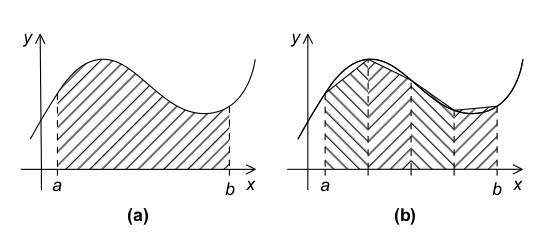
\includegraphics[width=0.7\textwidth]{trap.png}
    \end{center}  
\end{frame}
%------------------------------------------------------------------------------
\begin{frame}
  \frametitle{Aproximação trapezoidal}
  \begin{itemize}
    \item Área de um trapezoide $= \frac{h}{2}[f(x_i)+f(x_{i+1})]$
    \item $h = \frac{b-a}{n}$
    \item $x_0 = a$, $x_1 = a+h$, $x_2 = a+2h$, ..., $x_{n-1} = a+(n-1)h$, $x_n=b$
    \item Soma das áreas dos trapezoides:
  \end{itemize} 
  \begin{equation*}
    h[\frac{f(x_0)}{2}+f(x_1)+f(x_2)+....+f(x_{n-1})+\frac{f(x_n)}{2}]
  \end{equation*}
\end{frame}
%------------------------------------------------------------------------------
\begin{frame}
  \frametitle{Aproximação trapezoidal}
  \vspace{-5mm}
  \begin{center}
	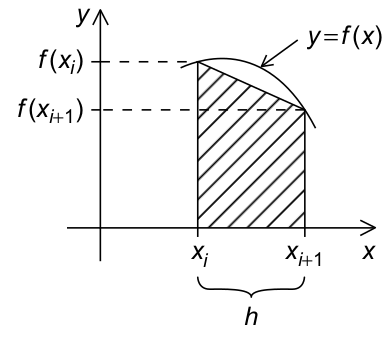
\includegraphics[width=0.4\textwidth]{trap1.png}
  \end{center}
  \vspace{-4mm}
  {\tiny An Introduction to Parallel Programming, Peter Pacheco, 2011.}
\end{frame}
%------------------------------------------------------------------------------
%------------------------------------------------------------------------------
\begin{frame}[fragile]
  \frametitle{Aproximação trapezoidal}
  Pseudo-código sequencial da aproximação trapezoidal.
\begin{center}
\begin{minipage}{0.95\textwidth}
  \begin{minted}[linenos, fontsize=\small, breaklines=true, frame=lines]{C}
/* Input: a, b, n */
h = (b - a)/n;
approx = (f(a) + f(b))/2.0;
for (i = 1; i <= n - 1; i++) {
  x i = a + i*h;
  approx += f(x i);
}
approx = h*approx;
  \end{minted}
\end{minipage}
\end{center}
\end{frame}
%------------------------------------------------------------------------------
\begin{frame}
  \frametitle{Aproximação trapezoidal paralela}
  \begin{itemize}
    \item Particionar o problema em tarefas.
    \item Identificar dependências entre tarefas.
    \item Agregar tarefas em tarefas compostas.
    \item Mapear tarefas compostas para processadores.
  \end{itemize} 
\end{frame}
%------------------------------------------------------------------------------
\begin{frame}[fragile]
  \frametitle{Aproximação trapezoidal paralela}
  Pseudo-código paralelo.
\begin{center}
\begin{minipage}{0.95\textwidth}
  \begin{minted}[linenos, fontsize=\small, breaklines=true, frame=lines]{text}
Get a, b, n;
h = (b - a)/n;
local_n = n/comm_sz;
local_a = a + my_rank*local_n*h;
local_b = local_a + local_n*h;
local_integral = Trap(local_a, local_b, local_n, h);
  \end{minted}
\end{minipage}
\end{center}
\end{frame}
%------------------------------------------------------------------------------
\begin{frame}[fragile]
  \frametitle{Aproximação trapezoidal paralela}
  Pseudo-código paralelo.
\begin{center}
\begin{minipage}{0.95\textwidth}
  \begin{minted}[linenos, fontsize=\small, breaklines=true, frame=lines]{text}
if (my_rank != 0)
  Send local_integral to process 0;
else /* my_rank == 0 */
  total_integral = local_integral;
  for (proc = 1; proc < comm_sz; proc++) {
    Receive local_integral from proc;
    total_integral += local_integral;
  }
}
if (my_rank == 0)
  print result;
  \end{minted}
\end{minipage}
\end{center}
\end{frame}
%------------------------------------------------------------------------------
%------------------------------------------------------------------------------
\begin{frame}
  \frametitle{Aproximação trapezoidal}
  \vspace{-5mm}
  \begin{center}
	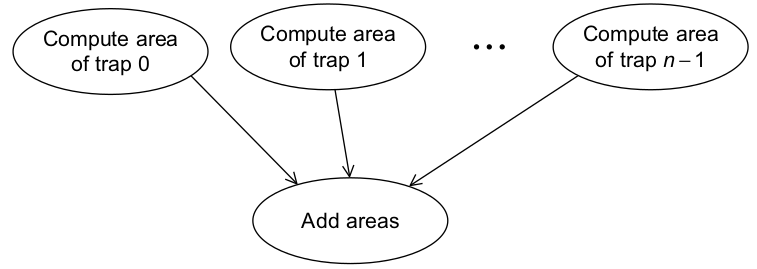
\includegraphics[width=0.8\textwidth]{trap2.png}
  \end{center}
  \vspace{-4mm}
  {\tiny An Introduction to Parallel Programming, Peter Pacheco, 2011.}
\end{frame}
%------------------------------------------------------------------------------
\begin{frame}[fragile]
  \frametitle{Aproximação trapezoidal sequencial}
\begin{center}
\begin{minipage}{0.95\textwidth}
  \begin{minted}[linenos, fontsize=\small, breaklines=true, frame=lines]{C}
double Trap(double a, double b, int n, double h) {
  double integral;
  int k;

  integral = (f(a) + f(b))/2.0;
  for (k = 1; k <= n-1; k++) {
    integral += f(a+k*h);
  }
  integral = integral*h;

  return integral;
}  /* Trap */   
  \end{minted}
\end{minipage}
\end{center}
\end{frame}
%------------------------------------------------------------------------------
% \begin{frame}[fragile]
%   \frametitle{Aproximação trapezoidal com MPI}
% \begin{center}
% \begin{minipage}{0.95\textwidth}
%   \begin{minted}[linenos, fontsize=\small, breaklines=true, frame=lines]{C}
% int main(void) {
%   int my_rank, comm_sz, n = 1024, local_n;   
%   double a = 0.0, b = 3.0, h, local_a, local_b;
%   double local_int, total_int;
%   int source; 
% 
%   MPI_Init(NULL, NULL);
%   MPI_Comm_rank(MPI_COMM_WORLD, &my_rank);
%   MPI_Comm_size(MPI_COMM_WORLD, &comm_sz);
% 
%   h = (b-a)/n;    
%   local_n = n/comm_sz; 
%   local_a = a + my_rank*local_n*h;
%   local_b = local_a + local_n*h;
%   local_int = Trap(local_a, local_b, local_n, h);
% 
%   /* Add up the integrals calculated by each process */
%   if (my_rank != 0) { 
%       MPI_Send(&local_int, 1, MPI_DOUBLE, 0, 0, 
%             MPI_COMM_WORLD); 
%   } else {
%       total_int = local_int;
%       for (source = 1; source < comm_sz; source++) {
%         MPI_Recv(&local_int, 1, MPI_DOUBLE, source, 0,
%             MPI_COMM_WORLD, MPI_STATUS_IGNORE);
%         total_int += local_int;
%       }
%   } 
% 
%   /* Print the result */
%   if (my_rank == 0) {
%       printf("With n = %d trapezoids, our estimate\n", n);
%       printf("of the integral from %f to %f = %.15e\n",
%           a, b, total_int);
%   }
% 
%   /* Shut down MPI */
%   MPI_Finalize();
% 
%   return 0;
% } /*  main  */
%   \end{minted}
% \end{minipage}
% \end{center}
% \end{frame}
%------------------------------------------------------------------------------
\begin{frame}[fragile]
  \frametitle{Aproximação trapezoidal com MPI}
\begin{center}
\begin{minipage}{0.95\textwidth}
  \begin{minted}[linenos, fontsize=\small, breaklines=true, frame=lines]{C}
int main(void) {
  int my_rank, comm_sz, n = 1024, local_n;   
  double a = 0.0, b = 3.0, h, local_a, local_b;
  double local_int, total_int;
  int source; 

  MPI_Init(NULL, NULL);
  MPI_Comm_rank(MPI_COMM_WORLD, &my_rank);
  MPI_Comm_size(MPI_COMM_WORLD, &comm_sz);
  \end{minted}
\end{minipage}
\end{center}
\end{frame}
%------------------------------------------------------------------------------
\begin{frame}[fragile]
  \frametitle{Aproximação trapezoidal com MPI}
\begin{center}
\begin{minipage}{0.95\textwidth}
  \begin{minted}[linenos, fontsize=\small, breaklines=true, frame=lines]{C}
  h = (b-a)/n;    
  local_n = n/comm_sz; 
  local_a = a + my_rank*local_n*h;
  local_b = local_a + local_n*h;
  local_int = Trap(local_a, local_b, local_n, h);
  \end{minted}
\end{minipage}
\end{center}
\end{frame}
%------------------------------------------------------------------------------
\begin{frame}[fragile]
  \frametitle{Aproximação trapezoidal com MPI}
\begin{center}
\begin{minipage}{0.95\textwidth}
  \begin{minted}[linenos, fontsize=\small, breaklines=true, frame=lines]{C}
  /* Add up the integrals calculated by each process */
  if (my_rank != 0) { 
      MPI_Send(&local_int, 1, MPI_DOUBLE, 0, 0, 
            MPI_COMM_WORLD); 
  } else {
      total_int = local_int;
      for (source = 1; source < comm_sz; source++) {
        MPI_Recv(&local_int, 1, MPI_DOUBLE, source, 0,
            MPI_COMM_WORLD, MPI_STATUS_IGNORE);
        total_int += local_int;
      }
  } 
  \end{minted}
\end{minipage}
\end{center}
\end{frame}
%------------------------------------------------------------------------------
\begin{frame}[fragile]
  \frametitle{Aproximação trapezoidal com MPI}
\begin{center}
\begin{minipage}{0.95\textwidth}
  \begin{minted}[linenos, fontsize=\small, breaklines=true, frame=lines]{C}
  /* Print the result */
  if (my_rank == 0) {
      printf("With n = %d trapezoids, our estimate\n", n);
      printf("of the integral from %f to %f = %.15e\n",
          a, b, total_int);
  }

  /* Shut down MPI */
  MPI_Finalize();

  return 0;
} /*  main  */
  \end{minted}
\end{minipage}
\end{center}
\end{frame}
%------------------------------------------------------------------------------

\begin{frame}[plain]{}
  \begin{center}
    \vspace{2cm}
    \Large{https://joao-ufsm.github.io/par2023a/}
    
    \vspace{1cm}
    
\includegraphics[width=2cm]{logo_ufsm}
    \hspace{0.5cm}
    
\includegraphics[width=2cm]{logo_inf}
  \end{center}
\end{frame}
%------------------------------------------------------------------------------

\end{document}
